% !TeX spellcheck = de_DE
% Metódy inžinierskej práce

\documentclass[10pt,oneside,slovak,a4paper]{article}

\usepackage[slovak]{babel}
%\usepackage[T1]{fontenc}
\usepackage[IL2]{fontenc} % lepšia sadzba písmena Ľ než v T1
\usepackage[utf8]{inputenc}
\usepackage{graphicx}
\usepackage{url} % príkaz \url na formátovanie URL
\usepackage{hyperref} % odkazy v texte budú aktívne (pri niektorých triedach dokumentov spôsobuje posun textu)
\usepackage{float}


\usepackage{cite}
%\usepackage{times}

\pagestyle{headings}

\title{Virtuálna realita vo vzdelavacom systéme\thanks{Semestrálny projekt v predmete Metódy inžinierskej práce, ak. rok 2020/21, vedenie: Martin Sabo}} % meno a priezvisko vyučujúceho na cvičeniach

\author{Patrik Kozlík\\[2pt]
	{\small Slovenská technická univerzita v Bratislave}\\
	{\small Fakulta informatiky a informačných technológií}\\
	{\small \texttt{xkozlik@stuba.sk}}
	}

\date{\small 1. november 2020} % upravte



\begin{document}

\maketitle

\begin{abstract}
Dnešná doba je primárne ovplyvnená vývojom technológii a novými výskummy z oblasti informatiky. Informatika stále káždým rokom zasahuje
viac do rôznych iných vedných oblastí. Počas tohoto rozvoja vnikla aj technológia virtuálnej reality, ktorá sa preslávila najmä vďaka jej
implemetácie do počítačových hier. Pri jej vývoji sa časom došlo na to, že by sa virtuálna realita dala zakomponovať aj do vzdelávania. 
Pri čom sa budem primárne zameriavať na jej implementáciu nie len do škôl, škôlok, zariadení pre ľudí so špeciálnymi potrebamy ale aj do múzeí. V závere uvediem vlastný návrh prepojenia virtualnej reality, múzea a študentov umeleckých vysokých škôl.   	
\end{abstract}



\section{Úvod}

Virtuálna realita v nedávnej dobe dosiahla veľkého rozmachu. Stala sa viac dostupná pre väčšie počty ľudí a hlavne čo je najdôležitejšie 
častejšie a častejšie sa s ňou začali stretávať aj obyčajný ľudia mimo IT sektoru. Vďaka tomu sa stala komerčná a dosiahla väčšej pozornosti,
čo znamená že dostala viac možností a financií na rozvoj. 

Avšak ohľadom virtuálnej reality v dnešnej dobe sa nám naskytáva otázka. Vieme že je využitá vo veľkom počte vďaka komercii ale je aj dostatočne využívaná vo vzdelavacom systéme na takej úrovni ako by mala byť?

Základom je zistenie výhod a nevýhod virtuálnej reality~\cite{Procon} aby sme vedeli s čím pracujeme a čo môže narušiť alebo urýchliť proces 
jej implementácie do vzdelávania.

Jednou z hlavných častí je už samotná implementácia virtuálnej reality do škôl, či do zariadení pre ľudí so špeciálnymi potrebamy,
kde môže byť veľmi prospešná a náučná.~\cite{VR}

No aby sme nezabudli vzdelávací proces neprebieha len v školách ale aj v múzeách, ktoré sú založené na približovaní histórie návštevníkovi, čo nám vie virtuálna realita predstaviť vizuálnou a zábavnejšou formou.

Potenciálnym prepojením virtuálnej reality v múzeách a vzdelávania v školách by sme mohli dosiahnuť veľmi žiaduce účinky na vzdelanosť študentov a zvýšiť ich motiváciu k štúdiu s pomocou tejto zábavnej a náučnej formy.

\section{Virtualna realita} \label{realita}
Virtualna realita je vcelku nová technológia, ktorá má v poslednej dobe stále viac a viac využití a jej potenciál do budúcnosti je obrovký. Je to technológia, ktorá vytvára simuláciu realisticky vyzerajúceho sveta, ktorý je obmedzený len predstavivosťou vývojára. V dnešnej dobe sa využíva primárne na zábavu najmä v spojení s poćítačovými hrami, no začína sa dostávať aj do vzdelávania. Túto technológiu tvoria 2 hlavné časti okuliare, ktoré nám podávajú zrakový vňem reality, a rukavie či ovládače, ktoré nám umožňujú interaktivitu s týmto svetom. Vývoj virtuálnej reality každým rokom napreduje a je len otázka času kedy nastane chvíľa a virtuálnu realitu nerozpoznáme od skutočnéjho sveta.~\cite{VR}  

\section{Výhody a nevýhody virtuálnej reality} \label{procon}
Pri využívaní virtuálnej reality je veľmi podstatná vedomosť o jej výhodách a nevýhodách. Ak chceme využiť virtuálnu realitu je veľmi podstatné aby sme vedeli s akými problémami sa môžeme stretnúť. Článok~\cite{Procon} nám tieto faktory bližšie upresnuje. Pri čom je zjavné, že virtuálna realita má viacej výhod ako nevýhod, čo je vidno aj v tabulke obrázok~\ref{tabulka}. No aj tak primárne záleží na tom v akom obore je využitá. Pár príkladov výhod a nevýhod si bližšie predstavíme. 

\subsection{Výhody} \label{procon:vyhody}
Pri výhodách sa nebudem zameriavať na jej výhody v hernom biznise ale skôr vo vzdelávaní. Hneď prvou a základnou výhodou je že prináša do vzdelávania simulácie ťažko predstaviteľných učív, pokusov, čo pomáha študentom pri lepšom zapamätávaní daného učiva či udrčiavaní ich pozornosti. Tieto simulácie sú dostatočne realistické na to aby podnietili emócie a donútili osobu konať v daných situáciách, pri čom podporuje kognitívne schopnosti. Pomocou tejto technológie vieme motivovať študentov a zväčšiť ich záujem o daný predmet výuky, pri čom im je tento predmet lepšie a pochopiteľnejšie predstavený. Už len s týchto príkladov vidíme, že je virtuálna realita prospešná a využiteľná technológia s potenciálom do budúcnosti.~\cite{Procon} 

\subsection{Nevyhody} \label{procon:nevyhody}
Nevýhody virtualnej realite mometálne nie sú až také početné, kedže nie sme ešte v dobe, kde by virtualna realita nahrádzala skutočný život, čo môže byť nevýhoda a problém o pár rokov. No v dnešnej dobe je jej najväčšia nevýhoda cena. Virtualna realita je vcelku drahá technológia a hlavne v momente ak ju chceme zakomponovať do vzdelávania. Už len ak si predstavíme zaobstarať príslušenstvo na VR pre jednu triedu 30 ľudí cena tejto investície bude dosť veľká, čo spôsobuje jej malú početnosť vo vzdelávaní.  

\begin{figure} 
	\centering
	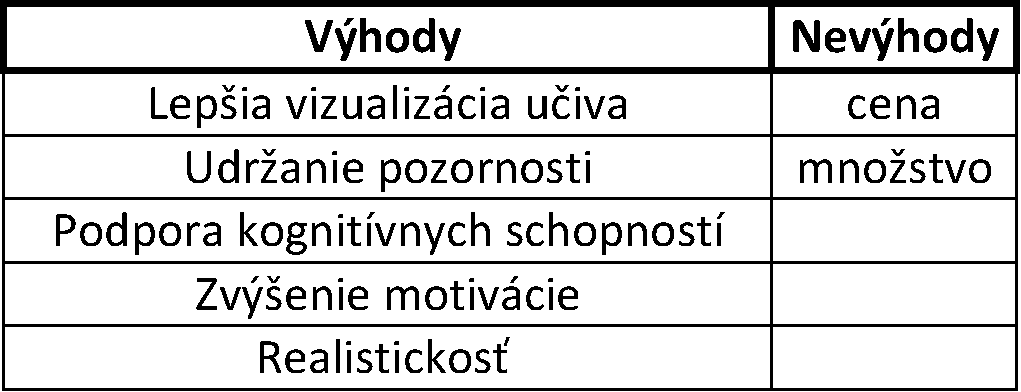
\includegraphics[width=10cm,height=6cm,keepaspectratio]{VR_tabulka-crop}
	\caption[VR_tabulka-crop]{Tabulka výhod a nevýhod virtualnej reality}
	\label{tabulka}
\end{figure} 

\section{Školy a pomocné zariadenia} \label{školy}
Už od začiatkov by s sme mali deti vzdelávať čo najlepšou a najprínosnejšou formou, jednou z nich je virtuálna realita. S jej pomocou môžeme dosiahnuť zábavnejší a lahšie memorizovatelnejší druh vzdelávania. No prospešná nieje len pre školy s normálnym zameraním ale je prospešná aj pre zariadenia so špeciálnym zameraním. 

\subsection{Školy} \label{školy:školy}
V základných školách sa virtuálna realita ešte len začína pomaly využívať a nieje bežným štandardom pre každú školu. Jedným z dôvodou sú financie, virtuálna realita nieje práve najlacnejšia technológia a nieje jednoduché zaobstarať triedu vybavenú touto technológiou. Avšak, myslím si že časom bude štandardom. Už teraz môžeme vidieť projekty ako je magic Mobius strip~\cite{Math} alebo 3D-VRLE~\cite{Physics}, ktoré vykazujú výsledky priamo zo škôl. 

Projekt magic Mobius strip~\cite{Math} je veľmi užitočný a prospešný návrh výučby matematiky, primárne geometrie, na zakladných školách. Projekt bol už v roku 2016 oskúšaný na pár zakladných školách v Číne, pri čom obdržal len pozitívne ohlasy. Klúčovou zložkou projektu je príslušenstvo, ktoré pozostáva z tabule, iPad ovládacieho systému, audia, VR okuliarov a vysielača VR siete. Pokus bol spravený na 32 študentoch vo veku od 10 do 12 rokov. Bolo viditeľné, že pri štúdiu geometrie niektrorí študenti nemali záujem, no v momente ako sa zapojil do výučby magic Mobius strip, všetko sa náhle zmenilo. Učili sa interaktívnou formou, mohli vytvárať vlastný útvar ,takzvaný mobiov list, a dokonca si aj zahrať interaktívnu hru.

Ďalšim úžasnym projektom je 3D-VRLE~\cite{Physics}. Projekt zameraný na fyziku, avšak pre zmenu sa tentoraz projekt zameriava už aj na zvýšenie motivácie pre daný predmet. Štúdiu uskutočnili spomedzi 65 študentiek, ktoré rozdelili na dve skupiny. Jedna skupina mala k dispozícii pri štúdiu bežné veci knihy, tabulu či prezentácie, no druhá skupina mala 3D-VRLE. Tento enviroment je tvorený balíkom digitálnych simulácii, animácii či interaktívnych demonštrácii fyziky vo virtuaĺnych laboraóriách. Pri študentoch, ktorý využívali 3D-VRLE bolo jasne preukázané zvýšenie nie len vedomostí, ktoré nadobudli a lepšie si zapamätali, ale aj zvýšenie záujmu o fyziku.

Podobných projektov, ktoré spájajú virtuálnu realitu a školy je mnoho. Toto sú len drobné príklady, no už len podľa týchto príkladov vieme povedať, že jej využívanie v školách má veľa benefitov od lepšieho zapamätávania učiva až po zvýšenie motivácie. Motivácia je nosným kameňom celého vzdelávanie. Ak by sme vedeli dobre implementovať virtuálnu realitu už v skorých rokoch štúdia na školách do bežnej výučby, mali by sme viac motivovaných študentov, ktorý by sa chceli vzdelávať v oblastiach, ktoré im táto virtuálna realita priblíži.  


\subsection{Zariadení pre ľudí so špeciálnymi potrebamy} \label{školy:zariadenia}
Virtuálna realita nemusí byť prospešná len v školách pri učení, no jej ďalšie úžasne využitie je aj na miestach kde by ste to naozaj neočakávali. Sú to zariadenia pre ľudí so špecialnymi potrebami. Jedným z príkladov sú osoby trpiace autizmom, ľudia čo trpia touto poruchou majú problémy s komunukáciou a socializáciou s okolím. No ak sa táto porucha indentifikuje a daný človek s ňou chce niečo spraviť sú možnosti ako. Práve jednou z možností je projekt half-CAVEAutism, ktorý využíva virtuálnu realitu na vzdelávanie týchto ľudí.

Tento úžasný projekt s názvom half-CAVE~\cite{Autism} nie je založený na rovnakých princípoch ako ostatné projekty. Nesnaží sa až v takej miere motivovať ako ostatné, no skôr pomáhať ľudom s autizmom pri ich adaptácii do bežného života. Projekt je tvorený 6 simuláciamy, ktoré človeka naučia ako zvládať emócie, stres v bežných situáciách ako je ranné vstávanie. Taktiež učia ako využívať relaxačné stratégie v napätých situáciach. No tento tréning nie je jednoduché zrealizovať, kvôli zložtosti virtuálneho prostredia. Prostredie potrebuje, jednu miestnosť, projektor, veľmi výkonný procesor a grafickú kartu, kameru, zrkadlo a pre priblíženie 128GB RAM. 

Ako vidíme virtualna realita je veľmi prospešná aj pri pomoci ľuďom so špecialnymi potrebami. Vďaka nej majú väčšiu možnosť na adaptáciu do normálneho života. Samozrejme človeka nevylieči úplne, ale už len tým že zlepší človeku kvalitu života, čo i len o trochu má veľký potenciál do budúcna. Momentálne tieto tréningy nie sú moc rozšírené, no ako budú časom ľudia zisťovať benefity tejto technológie budeme o nej frekventovanejšie počuť ako doteraz.   

\section{Virtuálna realita v múzeách} \label{muzea}
Pre niektorých ľudí a najmä mladšie generácie nie je jednoduché predstaviť si, ako to v minulosti fungovalo a vyzeralo. Mestá vyzerali inak, z dnešných zrúcanin boli hrady a niektoré miesta neboli vôbec osýdlené. No ohľadom histórie máme veľa záznamov, ktoré nám vedia pribížiť, ako minulosť vyzrala. Prepojením týchto záznamov, 3D dizajnérov a odborníkov na VR viemem dosiahnuť úžasné výsledky. Vieme zrekonštruovať nie len malé miestnosti ale aj celé domy či dokonca celé oblasti. Avšak neexistuje len rekonštrukcia predmetov, stavieb a oblastí ale aj živočíchov, ktoré nám dokážu priblížiť život v minulosti. Vďaka tomu, že ľudia zistili že je náučnejšie tieto veci vidieť a nie len o nich počuť začala sa v múzeách využívať virtuálna realita.

Jedným z príkladov využitia tejto technológie je múzeum na ostrove Rhodos~\cite{Muzeum}. Toto múzeum využíva technológiu úžasnym spôsobom. Zozbieralo, vytvorilo a vložlo okolo 150 objektov do virtuálneho sveta.Tento svet obsahoval 7 častí predstavujúcich umenie, náboženstvo, obranu a vrstvy obyvateľstva. Pri čom tento enviroment vložili do 3 interaktívnych miestností. Fascinujúcou časťou projektu je, že aplikáciu vytvorili iba za 345 hodín a snažli sa pri tom využiť čo najmenej financii, pričom aplikácie bežali na 5 rokov starých počítačoch.

Využitie virtualnej reality v múzeách je veľmi dôležité a dokážeme ju interaktívne použiť. Dokáže nám odprezentovať minulosť takým spôsobom ako by sme v tej danej dobe práve boli a videli predmety, ktoré už dávno neexistujú.  Dáva nám možnosť vzdelávať nie len študentov ale aj návšteníkov múzea. No úžasné je, že aj s týmito limitmy, ktoré mal tento projekt, dokázali tvorcovia vytvoriť funkčný a náučný software s využitím virtualnej reality. Toto dáva nádej, že virtalnu realitu bude možné využiť aj v školách a múzeách s menšími finančnými prostriedkami.



\section{Virtuálna realita v múzeách v spojení so sochárstvom} \label{produkt}

Ako som už načrtol, virtuálna realita v múzeách je dosť využívaná a vie nám veľmi dobre a s veľkou presnosťou zobraziť predmety v digitálnej forme. Dané prepojenie virtuálnej reality, múzea a sochárstva, ktoré navrhujem slúži primárne pre študentov sochárstva no môže byť taktiež veľmi prospešné aj pre maliarov či iných umelcov. Prepojenie ľudí a projektu je vyzobrazené v grafe~\ref{diagram}. Základom projektu je miestnosť s virtuálnou realitov. No to nie je stavebným kameňom projektu. Najdôležitejšou časťou je software obsahujúci dve primárne zložky. Prvá zložka by obsahovala 3D skeny skutočných ľudí, pri čom niektoré by boli zamerané na telo a iné na výraz tváre človeka. Druhou zložkou by boli 3D skeny najznámejších sôch na svete, vďaka čomu by si kdokoľvek a kdekoľvek mohol pozrieť tieto známe diela. Po nasadení 3D okuliarov by sa nami vybratý model zobrazil v strede miestnosti a mohli by sme si ho pozrieť z blízkosti akej budeme chcieť, či s nami vybraného uhla. Pri výuke maliarov, či sochárov by to bol veľmi užitočný nástroj. Ja sám sa zaujímam o 3D modelovanie, pri čom štúdium anatómie je veľmi zložité len z referenčných 2D obrázkou. S pomocou tohoto softwaru by sme boli schopný s využitým malých financií pomôcť umelcom pri štúdiu. Mimo hodín výuky študentov by sa dala táto technológia použiť pre návštevníkov múzea, ktorý by si mohli prezrieť v tejto miestnosti modely známych pamiatok ako je Koloseum či Sochu slobody z bezprostrednej blízkosti. Jedinou zložitou časťou by bolo vytvorenie skenov, ktorých by muselo byť obrovské množstvo, no ak by sme ich dokázali získať mali sme prístup k dielam najznámejších umelcov, pri čom by sme nemuseli ani len opustiť mesto v ktorom práve budeme. 
 
 \begin{figure}[H]
 	\centering
 	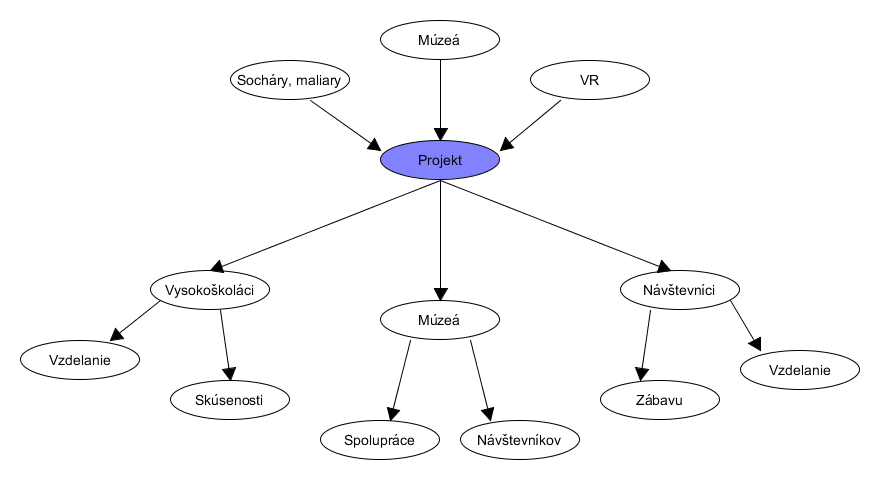
\includegraphics[width=18cm,height=6cm,keepaspectratio]{diagram}
 	\caption[diagram]{Diagram prepojenia virtualnej reality a umenia}
 	\label{diagram}
 \end{figure} 

\section{Záver} \label{zaver} % prípadne iný variant názvu

Ako poukazuje článok virtuálna realita má mnoho využití vo vzdelávaní. Je dokázateľne prospešná nie len pre študentov, ale aj pre ľudí s postihnutím, či obyčajných ľudí. Pomáha pri výuke, vzdelávaní, či aklimatizácii ľudí. No táto technológia nie je využitá tak ako by mohla byť. Ak by sa dokázala virtualna realita implemetovať do škôl, ako štandart, časom by sa objavili viditeľné výsledky a pozitíva na študentoch a obyčajných ľuďoch, ktorým by sa zvýšili vedomosti a záujem. Preto si myslím, že virtuálna realita v budúcnosti dosiahne svojho právoplatného miesta a budeme sa s ňou stretávať viac ako si teraz myslíme.

\paragraph{Spoločenské súvislosti.}V dnešnej dobe virtualna realita nie je vo vzdelávacom systéme vo veľkom počte, ale aj tak vieme povedať, že spoločnosť ovplyvňuje a bude stále viac a viac ovplyvňovať tak ako každá jedna technológia na tomto svete. S jej rozširovaním v systéme príde taktiež nový druh výuky, ktorý bol spomenutý v projektoch~\cite{Math}~\cite{Physics}. Tento druh výuky zmení od základov štýl štúdia a teda aj spoločnosť, ktorá na ňu naväzuje. A je len na nás, či zmení spolčnosť na vzdelanejšiu alebo nevzdelanejšiu.  

\paragraph{Historické súvislosti.}Málokto by povedal, že prvý krát sa ľudstvo stretlo s virtualnou realitou už v roku 1962. Od tej doby prešla veľkým vývojom, využila sa vo veľa odvetviach a ovplyvnila históriu. Využívala sa a stále sa využíva pri tréningu vojakov, no taktiež sa využíva pri simuláciách v oblasti medicíny či dopravy. Tieto využitia mali veľký význam pre náš dnešný svet, pretože ho zmenili do podoby, ktorú vidíme teraz. Pri čom pomohli pri vývoji nových technológii a zachránila nespočetne životov.  

\paragraph{Technológia a ľudia.}Ľudia sú bezpochyby s virtuálnou realitou silne prepojený. Ako ju človek využíva na vzdelávanie tak ju využíva aj na zábavu. Dokáže taktiež mnohým ľudom pomôcť so zdravotnými problémamy ako sme videli v článku~\cite{Autism}. Vypomáha učiteľom, architektom, letcom, vojakom a mnohým ďalším, ktorým ulahčuje prácu a pripravuje ich na zdanlivo nenatrénovateľné situácie. No taktiež prináša zábavu a realistické zážitky obyčajným ľudom, čo robí s virtuálnej reality nástroj pre každého. 

\paragraph{Udržateľnosť a etika.}Z hladiska udržateľnosti je virtuálna realita bezproblémová, vďaka jej obrovskému potenciálu do budúcnosti je jej vývoj v dnešnej dobe nezvyčajne rýchly a pokrokový. Avšak problém nastáva pri etike, čím realistickejšia virtuálna realita bude, tým väčší problém s etikou nastane. Od osôb, ktoré budú vo virtuálnej realie až po aktivity, ktoré sa v nej budú vykonávať. Virtuálna realita je dnes stále len na začiatku, no s tempom akým rastie môže rýchlo naraziť na barieru, ktorá sa nebude týkať technológie ale práve etiky. 

%\acknowledgement{Ak niekomu chcete poďakovať\ldots}


% týmto sa generuje zoznam literatúry z obsahu súboru literatura.bib podľa toho, na čo sa v článku odkazujete
\bibliographystyle{unsrt} % prípadne alpha, abbrv alebo hociktorý iný
\bibliography{literatura}
\end{document}
